\chapter{Speicher}

\section{Moderne File Systeme}

\subsection{Sie wissen was ein modernes Filesystem leisten muss.}

Ein modernes Filesystem sollte folgende Anforderungen erfüllen:
\begin{itemize}
	\item grosse Adressierbarkeit
	\item Volume Manager eingebaut
	\item umfangreiche Funktionalitäten
	\item immer konsistent und integer
	\item kein fsck mehr nötig nach Absturz
	\item kann mit \emph{silent corruption} umgehen (unabsichtliche Änderungen von Bits)
\end{itemize}
Ein schon etwas in die Jahre gekommenes Filesystem ist das Unix File System (UFS). Im UFS werden Daten in Blöcken abgelegt und alle Informationen zu einer Datei sind in sogenannten \texttt{inodes} abgelegt. Das Dateisystem ist hierarchisch aufgebaut wobei die Hierarchiestufen Verzeichnisse, Dateien oder Laufwerke sein können. UFS hat ein paar Nachteile s können in der aktuellen Version nur 1 TB adressiert werden und auch fsck muss nach einem Absturz ausgeführt werden.

Ein Beispiel für ein modernes Filesystem ist ZFS welches von Sun Microsystems entwickelt wurde. Eine gute Übersicht bietet dieser Artikel: \href{http://www.admin-magazin.de/Online-Artikel/ZFS-Snapshots-RAID-und-Datensicherheit}{http://www.admin-magazin.de/Online-Artikel/ZFS-Snapshots-RAID-und-Datensicherheit}

\subsection{Sie wissen wie ein modernes Filesystem aufgebaut ist.}

\subsubsection{Volumes vs. Pooled Storage}

Bei traditionellen Filesystemen war ein Filesystem für eine physikalische Partition zuständig. Wollte man mehrere physikalische Partitionen zu einer logischen Partition zusammenfassen musste man zusätzlich einen Logical Volume Manager installieren. Durch logische Volumen kann man z.B. Speicherplatz von zwei Festplatten zusammenfassen oder ein Volume spiegeln.
ZFS fasst diese Funktionen zusammen indem die physischen Datenträger (alles vom Floppy bis zur SSD) in einem Pool zusammengefasst werden. Aus diesem Pool können das beliebig viele logische Partitionen mit eigenem Dateisystem erstellt werden. Die logischen Partitionen können dynamisch wachsen oder durch den Admin eingeschränkt werden.
Klassische Dateisysteme abstrahieren zwar die Festplattenlogik, müssen dadurch aber komplizierte Strukturen erstellen um die Dateien abzuspeichern (kostet Zeit). ZFS verwendet zur Speicherung von Dateien und Metadaten ZFS-Objekte welche die DMU (Data Management Unit) zur Verfügung stellt. Wird nun eine Schreiboperation vom Betriebssystem ausgelöst, startet die DMU eine Transaktion. Gleichzeitig abschliessende Transaktionen werden zu Transaktionsgruppen gesammelt und dem SPA (Storage Pool Allocator) übergeben, welcher sie auf die physikalischen Platten schreibt.

\subsubsection{Konsistenz}

Nach einem Systemzusammenbruch kann das Filesystem in einem inkonsistenten Zustand sein, insbesondere wenn Blöcke für die Dateiverwaltung nicht korrekt auf die Festplatte geschrieben wurden. Mittels \texttt{fsck} wird ein Konsistenztest auf File- und Blockebene durchgeführt (Blöcke weder frei noch File zugeordnet, Block tritt mehrfach auf usw.). \texttt{fsck} kann bei grossen Dateisystemen sehr lange dauern und man möchte ständig wissen ob die Daten korrupt sind. Um jederzeit konsistent zu sein können Dateien auf zwei Arten geschrieben werden:
\begin{description}
	\item[CoW (Copy On Write):] Die alten Daten werden in einen neuen Speicherblock kopiert. Die Daten im alten Speicherblock werden überschrieben mit den neuen Daten.
	\item[RoW (Redirect On Write):] Neue Schreibanfrage möchte die Daten in den alten Block schreiben. Diese werden aber in einen neuen Block geschrieben (redirect). Der Originalblock enthält alte Daten.
\end{description}
ZFS verwendet CoW obwohl es eher ein RoW ist. Abbildung \ref{fig:write-file-zfs} zeigt wie eine Datei im ZFS geschrieben wird. Nachfolgend sind die einzelnen Schritte beschrieben:
\begin{enumerate}
	\item Man geht vom konsistenten Zustand aus, bei dem das Filesystem mit den blauen Blöcken vollständig in Ordnung ist. Die Daten liegen dabei nur in den Blättern des Baumes. Die inneren Knoten des Baumes enthalten lediglich Zeiger und keine sonstigen Daten. Die separat gespeicherte Wurzel des Baumes heisst bei ZFS Überblock.
	\item Nun sind ein paar Dateien zu schreiben. ZFS sucht dafür freie, momentan unbenutzte Blöcke (im Bild sind diese Blöcke grün hervorgehoben), es überschreibt niemals belegte. Ausserdem achtet es darauf, dass die Blöcke möglichst beieinander liegen, um effizient schreiben zu können. Noch gelangen die Daten aber nicht auf die Platte, weil sonst die Transaktion nicht mehr rückgängig zu machen wäre.
	\item Irgendwann schliesst das Betriebssystem die Transaktion ab (commit). Dazu ist der Baum bis zur Wurzel zu aktualisieren. Der linke Block in der mittleren Ebene erhält die Zeiger auf die beiden neuen Datenblöcke. Der linke Block auf der Ebene darüber erhält links den Zeiger auf den eben modifizierten Block, und rechts wird der unveränderte Teil eingetragen. Dieser Schritt fasst in der Regel mehrere Schreibvorgänge in einer so genannten Transaktionsgruppe zusammen.
	\item Nun ist alles vorbereitet, um die Transaktion endgültig zu beenden. Dazu schreibt ZFS den Überblock (im Bild: kleines Quadrat). Ist der neue Überblock erzeugt, sind die eben erstellten Blöcke im Filesystem aktiv. Bricht das System aus irgendeinem Grund ab (»halt«-Kommando an der Konsole, Systemabsturz, Stromausfall, ...), dann existiert noch der alte Überblock und damit der alte Zustand in den blauen Blöcken, denn das Filesystem beschrieb lediglich Blöcke, die im Ausgangszustand (blau) unbenutzt waren.
\end{enumerate}
\begin{figure}
\centering
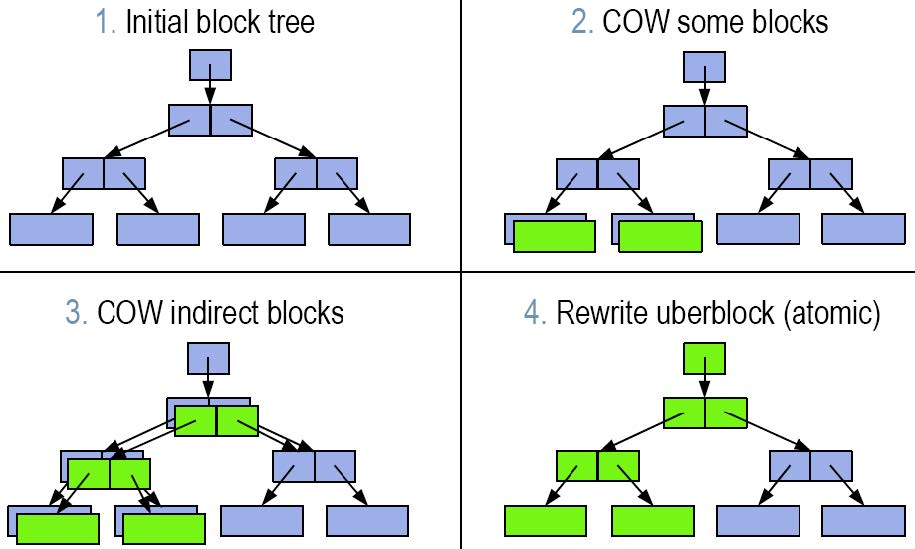
\includegraphics[width=0.7\linewidth]{fig/write-file-zfs}
\caption{Datei schreiben in ZFS}
\label{fig:write-file-zfs}
\end{figure}
Wenn beim schreiben des Überblocks etwas schiefgeht hat ZFS auch diverse Mechanismen auf Lager um ihn wiederherzustellen.

\subsubsection{Snapshots}

Snapshots bezeichnen eine Kopie eines Filesystems zu einem bestimmten Zeitpunkt, die nicht mehr veränderlich ist. In ZFS lässt sich ein solcher Snapshot sehr einfach herstellen: Man merkt sich lediglich den Zeiger auf den Wurzelknoten des Filesystems und hat damit den Snapshot ohne grossen Aufwand bereits realisiert. Da bei Änderungen nie Datenblöcke überschrieben werden, kann der Snapshot weiterhin die alten Datenblöcke referenzieren. Wird eine Datei verändert und möchte man diese in den Snapshot übernehmen muss lediglich die Referenz geändert werden (Abbildung \ref{fig:snapshot}).

\begin{figure}
\centering
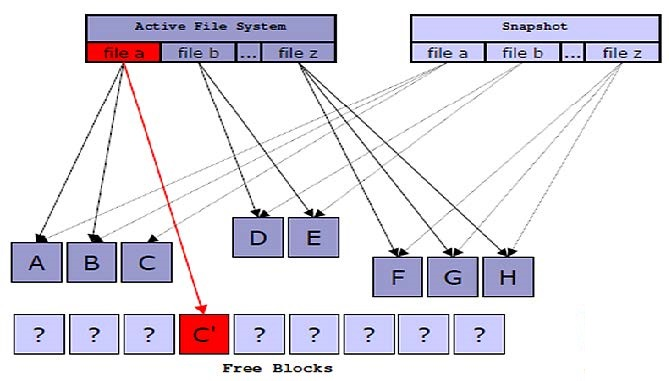
\includegraphics[width=0.7\linewidth]{fig/snapshot}
\caption{Snapshot}
\label{fig:snapshot}
\end{figure}

\subsubsection{Selbstheilung}

Herkömmliche Filesysteme setzen auf Sektorprüfsummen und RAID um Datenverlust zu verhindern. Diese Techniken erkennen aber eine ganze Reihe von Fehlern nicht. ZFS kann Daten selbstständig redundant speichern (RAID 1) und beherrscht auch eine verbesserte RAID 5-Variante welche sich RAID z nennt. Zusätzlich zu diesen bekannten Techniken kann sich ZFS selbst heilen. Wenn ein herkömmliches Filesystem einen defekten Block liest bleibt das unbemerkt, auch wenn eine Spiegelung des defekten Blockes vorhanden ist. Der defekte Block wird dann vom User Prozess verarbeitet, was zu Systemabstürzen führen kann. ZFS erkennt solche defekten Blöcke zur Laufzeit mittels Prüfsumme und ersetzt den defekten Block mit seiner Spiegelung auf einem anderem Device. Zusätzlich kann ZFS den defekten Block auch reparieren. Dieser Vorgang muss jedoch manuell ausgelöst werden.

\subsection{Sie wissen wie der Kern und das File System zusammenarbeiten.}

\subsubsection{Buffer Cache}

Wenn ein Prozess auf Datenblöcke eines Files zugreifen will, so bringt der Kern diese Blöcke in den Hauptspeicher, ändert diese nach Bedarf und macht danach eine Anfrage diese im File System zu speichern (z.B. \texttt{cp fileone.c filetwo.c}). Um den Durchsatz zu erhöhen richtet der Kern beim Systemstart einen sogenannten Buffer Cache ein. Der Buffer Cache ist eine Softwarestruktur welche den Durchsatz drastisch erhöhen kann. Der Datentransfer zwischen dem Buffer Cache (Kern-Raum) und dem User Prozess-Raum wird immer über DMA (Direct Memory Access) gemacht, weil so keine Prozessor-Zyklen verbraucht werden.
Ein Buffer besteht aus zwei Teilen:
\begin{description}
	\item[Memory Array:] Speicherblöcke
	\item[Buffer Header:] Kopf eines Speicherblockes mit Metadaten
\end{description} 
Der Buffer Header hat ca. 20 Einträge. Die folgenden Einträge kennzeichnen den Datenblock im Memory Array:
\begin{description}
	\item[Device Nummer:] ID vom angeschlossenen Gerät (Harddisk, USB-Stick usw.)
	\item[Block Nummer:] ID von Daten auf der Disk
	\item[Status vom Block:] Buffer gesperrt, Buffer enthält gültige Daten, verzögertes Schreiben, Kern liest/schreibt Inhalt, Prozess wartet bis Buffer frei wird
\end{description}
Der Kern identifiziert den Bufferinhalt indem er die Device- und Blocknummer überprüft. Der Kern unterhält zwei doppelt verknüpfte Listen. Eine \emph{Freie Liste} in welcher alle freien Buffer eingetragen sind und eine Hash-Queue (Hash über Device- und Blocknummer) welche verwendet wird um auf einen Disk Block zuzugreifen.

%TODO Buffer Szenarien (bin nicht drausgekommen).

\subsubsection{Virtual File System (VFS)}

Das VFS ist eine Abstraktion des zugrundeliegenden Filesystems und bietet eine einheitliche Schnittstelle für die Dateimanipulation einem User Prozess an. Die Schnittstelle kann von einem User Prozess im POSIX Format angesprochen werden (z.B. \texttt{open( „/usr/include/unistd.h“, O\_RDONLY)}) Das VFS setzt voraus dass ein File einen einzigartigen Namen und einen Benutzer hat. Für jedes spezifische Filesystem wird ein Mapping Modul bereitgestellt welches das reelle Filesystem auf das virtuelle Filesystem transformiert. Auf der Abbildung \ref{fig:virtual-file-system} ist dieses Mapping im Detail abgebildet.

\begin{figure}
\centering
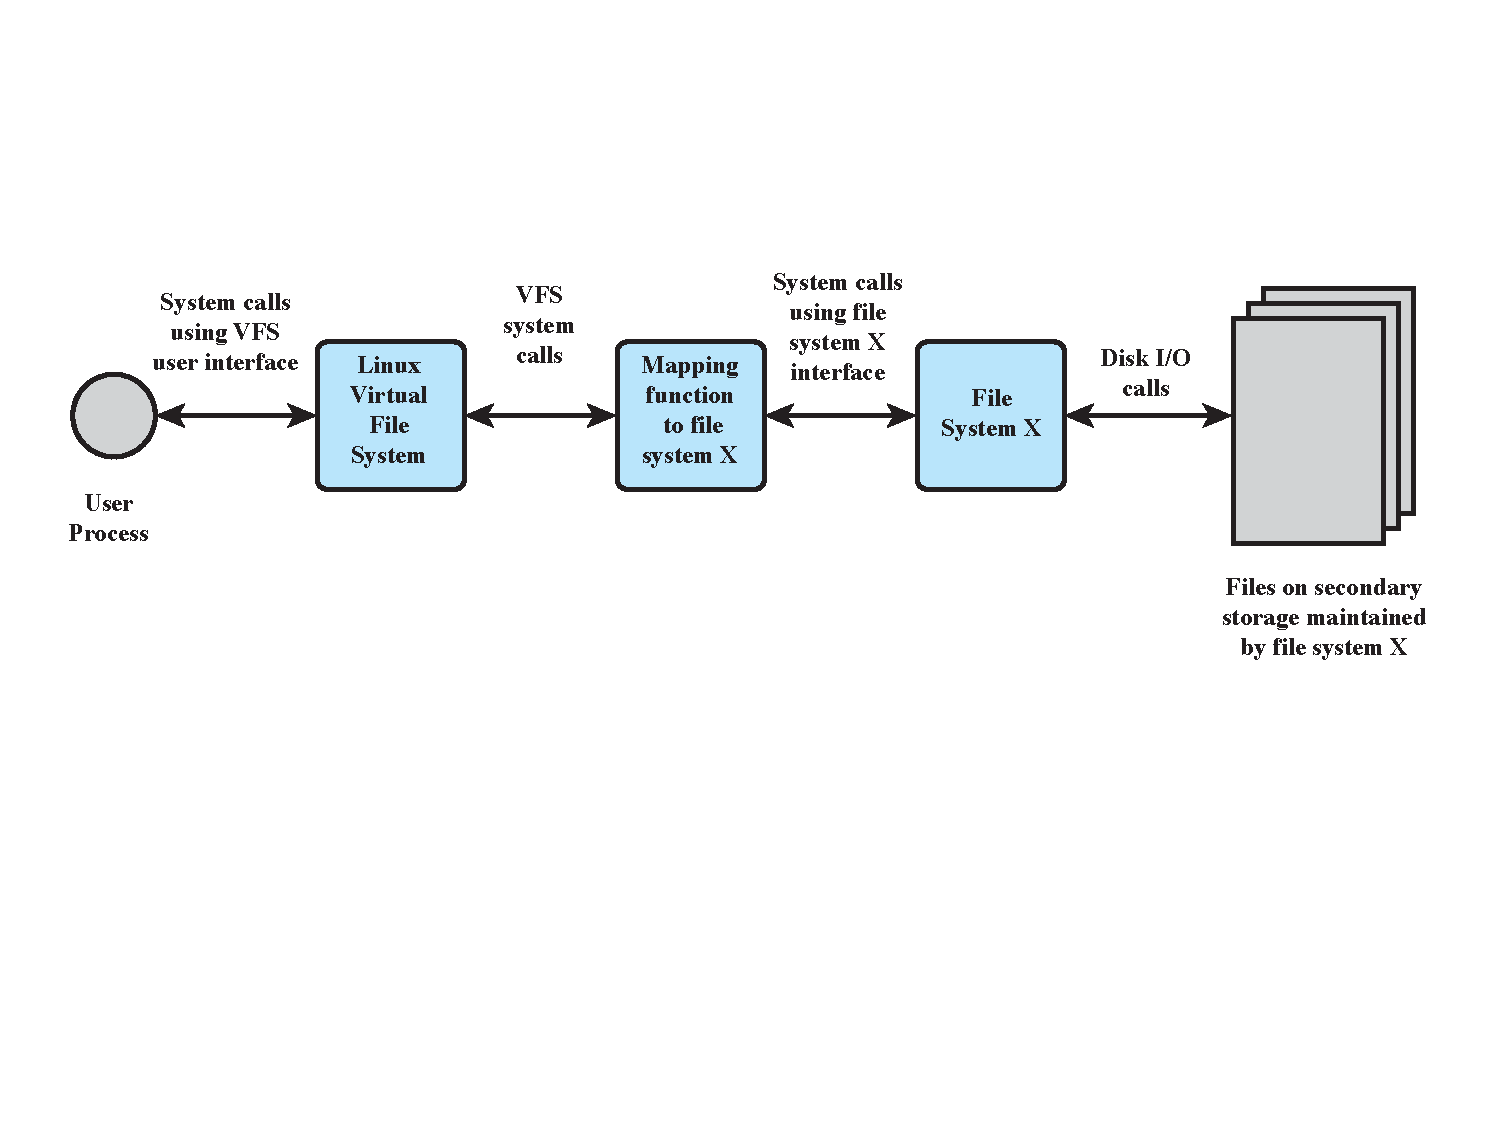
\includegraphics[width=0.7\linewidth]{fig/virtual-file-system}
\caption{Virtual File System}
\label{fig:virtual-file-system}
\end{figure}

\subsection{Sie kennen die internen Strukturen eines Filesystems.}

Das ZFS ist in einer Baumstruktur (Merkle Tree) aufgebaut. Der Wurzelknoten wird \emph{Uberblock} genannt. Die Knoten zwischen dem \emph{Uberblock} und den Blättern enthalten Block Pointers. Block Pointer enthalten \emph{Data Virtual Addresses} zu anderen Blöcken und zusätzlich auch den Hash von seinen Kind Knoten. Die Blätter des Baumes enthalten dann die eigentlichen Daten.

\section{Speichernetze \& Protokolle}

\subsection{Sie wissen wie ein Storage Area Network aufgebaut ist.}

Zurzeit sind folgende Speicherprotokolle weit verbreitet:
\begin{description}
	\item[SCSI:] altes \emph{Small Computer Serial Interface}
	\item[SAS:] neues \emph{Serial Attached SCSI} (abwärtskompatibel zu SATA)
	\item[SATA:] für billig Produkte, hat Limitationen
\end{description}
In einem SAN müssen die Befehle eines dieser Speicherprotokolle über das Netzwerk übertragen werde. Bekannte Transportprotokolle sind:
\begin{description}
	\item[Fibre Channel:] Überträgt SCSI-Befehle
	\item[TCP/IP:] Überträgt SCSI-Befehle über TCP (wird meist in KMU's verwendet)
\end{description}
Die SCSI-Kommandos werden in folgende vier Kategorien eingeteilt:
\begin{description}
	\item[N] non-data
	\item[W] Schreiben der Daten vom Initiator zum Target
	\item[R] Lesen der Daten
	\item[B] Bidirektional
\end{description}
Abbildung \ref{fig:scsi-read} zeigt ein Beispiel für den Read Befehl von SCSI. Dabei sind folgende Elemente interessant:
\begin{description}
	\item[Operation Code:] Der Hexcode 08 steht für den Read Befehl
	\item[Logical Unit Number (LUN):] Die LUN ist eine Nummer um eine durch das SCSI Protokoll adressierte logische Diskeinheit zu identifizieren. Eine LUN wird für jegliche Geräte verwendet, egal ob Tapes oder virtuelle Volumes.
	\item[Logical Block Address (LBA):] Die LBA ist die Startadresse von welcher man einen Block lesen möchte.
	\item[Transfer Length:] Die Transfer Length gibt die Anzahl der Blöcke an, die man lesen möchte.
\end{description}

\begin{figure}
\centering
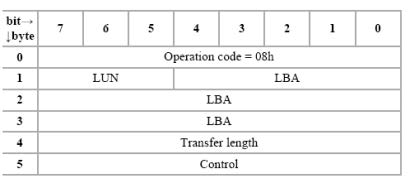
\includegraphics[width=0.7\linewidth]{fig/scsi-read}
\caption{SCSI Read Befehl}
\label{fig:scsi-read}
\end{figure}

Abbildung \ref{fig:fc-topologien} zeigt eine Überblick über die verschiedenen Fibre Channel Topologien. Von den drei Topologien hat sich nur die Fabric Topologie durchgesetzt. 

\begin{figure}
	\centering
	\begin{subfigure}[b]{0.3\textwidth}
		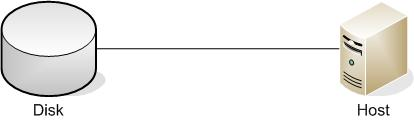
\includegraphics[width=\textwidth]{fig/fc-point-to-point}
		\caption{Point to Point}
	\end{subfigure}
	~
	\begin{subfigure}[b]{0.3\textwidth}
		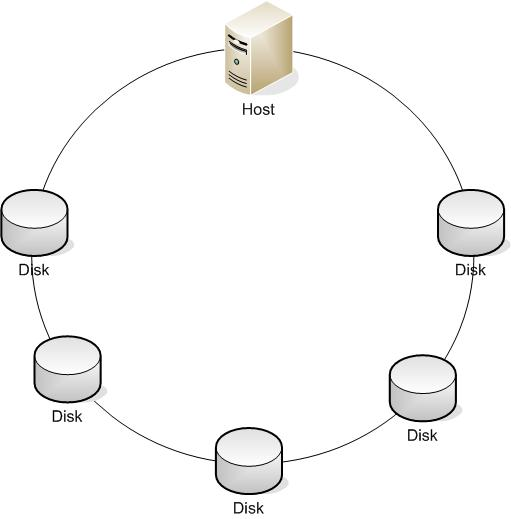
\includegraphics[width=\textwidth]{fig/fc-loop}
		\caption{Loop}
	\end{subfigure}
	~
	\begin{subfigure}[b]{0.3\textwidth}
		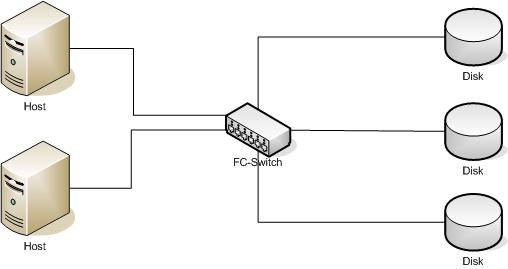
\includegraphics[width=\textwidth]{fig/fc-fabric}
		\caption{Fabric}
	\end{subfigure}
	\caption{Fibre Channel Topologien}\label{fig:fc-topologien}
\end{figure}

Bei der Fabric Topologie werden die Server und die Storage Subsysteme an einen Fibre Channel Switch angeschlossen. Fibre Channel mit einer Fabric Topologie umgesetzt bietet folgende Vorteile:
\begin{itemize}
	\item Mehrzweck-Netzwerk möglich um Speichergeräte, Video Streaming und Cluster Server zu verbinden.
	\item Transportiert Protokolle (SCSI, IP usw.) von einer höheren Ebene (yet-another-new-protocol).
	\item Hochgeschwindigkeiten von bis zu 16 Gbit/sec (2015).
	\item Kollisionsfreie Übertragung.
	\item Reichweite von bis zu 10 km (mit Extender mehr möglich für Disaster Recovery).
	\item Fortschrittliches System der Fluss Kontrolle.
	\item Unterstützt Heterogene Systeme (Linux, Solaris, Vmware, Citrix usw.)
\end{itemize}
Eine SAN Fabric besteht aus folgenden Hardware-Komponenten:
\begin{description}
	\item[Host Bus Adapter:] Der Host Bus Adapter stellt die Schnittstelle zwischen dem internen Server-Bus (z.B. PCIe) und dem FC Netzwerk zur Verfügung.
	\item[Verbindungskabel:] Als Verbindungskabel können Kupfer- oder Glasfaserkabel verwendet werden.
	\item[GBIC (Gigabit Interface Converters):] Dieser Adapter können im Host Bus Adapter oder im Fibre Channel Switch eingesetzt werden und stellen die Medien-Schnittstelle (Kupfer zu Glas) bereit.
	\item[SFP (Small Form Factor Pluggable):] Die SFPs sind eine Weiterentwicklung der GBIC und unterscheiden sich vor allem in ihrer kompakteren Bauweise.
	\item[Fibre Channel Switch:] Leiten die Datenpakete mit einem Cut-Through Routing weiter (ohne Zwischenspeichern). Dadurch kann ein FC Switch ein Frame in 2-4 Mikrosekunden verarbeiten.
	\item[Storage Subsystem:] Das Storage Subsystem stellt den Speicher in verschiedener Form (SSD, Tape usw.) bereit.
\end{description}

\subsection{Sie kennen das FC Protokoll und dessen Eigenschaften.}

Jedes Gerät im FC Netzwerk besitzt einen 64 bit langen \emph{Node Name}. Jeder Port an diesem Gerät besitzt zudem einen 64 bit langen \emph{Port Name}. Für das Routing wird zusätzlich pro Port eine 24 bit lange \emph{N\_Port ID} als Adresse verwendet.
Das FC Protokoll besteht aus 5 Layer welche nachfolgend genauer beschrieben sind:
\begin{description}
	\item[FC-4 (Protocol Mapping Layer):] Im Protocol Mapping Layer werden Anwendungsprotokolle, wie z.B. SCSI oder IP in eine Protocol Data Unit verpackt, damit diese über den FC-2 Layer zugestellt werden kann.
	\item[FC-3 (Common Services Layer):] Im Common Services Layer können erweiterte Funktionen wie beispielsweise RAID-Absicherung oder Verschlüsselung implementiert werden.
	\item[FC-2 (Network Layer):] Der Network Layer stellt den eigentlichen Kern des FC-Protokolls dar.
	\item[FC-1 (Data Link Layer):] Im Data Link Layer ist die Umsetzung der Daten in Leitungssignale implementiert.
	\item[FC-0 (Physical):] Der Physical Layer, der die Verkabelung, Stecker und Steckertypen usw. definiert.
\end{description}
Um einer grossen Anzahl von Ansprüchen in der Kommunikation gerecht zu werden, definiert FC mehrere Service Klassen im FC-2 Layer. Abbildung \ref{fig:fc-service-classes} gibt einen Überblick über alle Klassen. 

\begin{figure}
\centering
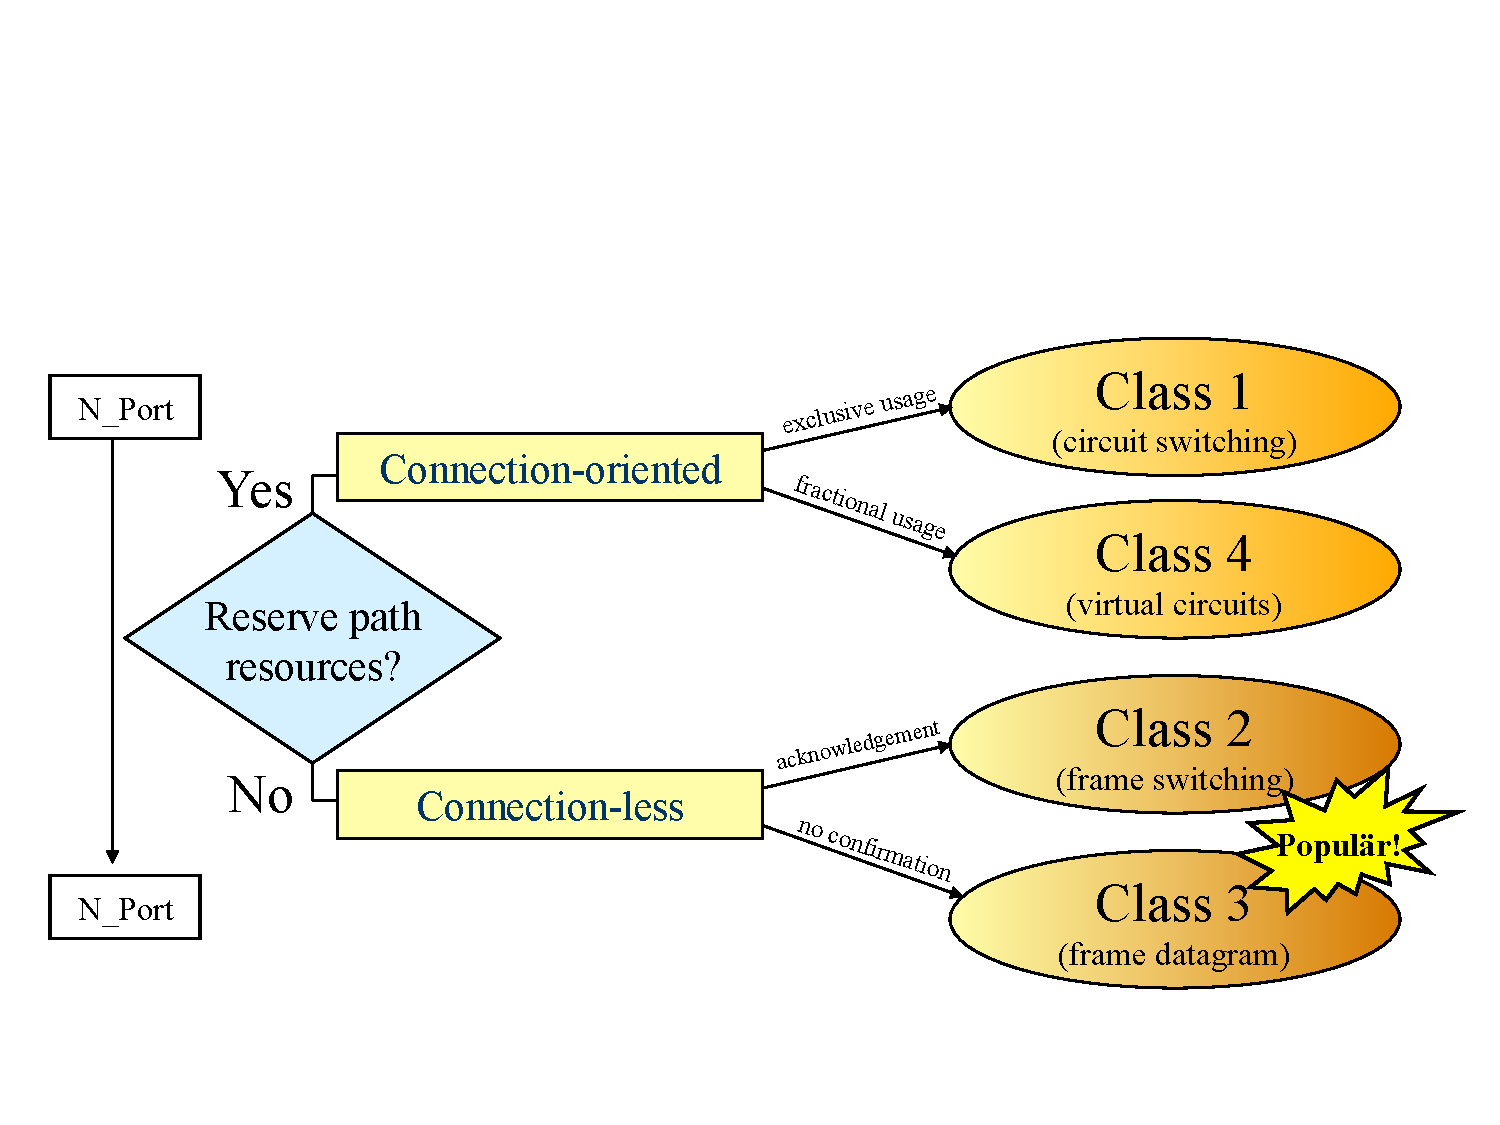
\includegraphics[width=0.7\linewidth]{fig/fc-service-classes}
\caption{Fibre Channel Service Klassen}
\label{fig:fc-service-classes}
\end{figure}

Fibre Channel definiert verschiedenen Port Typen. Bei einem Gerät (Server, Storage usw.) gibt es folgende zwei Ports:
\begin{description}
	\item[N\_PORT:] Das Gerät ist direkt mit einem Switch verbunden.
	\item[NL\_PORT:] Das Gerät ist in einer Loop Topologie verbunden.
\end{description}
Bei einem Switch werden folgende Ports definiert:
\begin{description}
	\item[U\_Port:] Universal Port (verwendet für automatische Port Erkennung).
	\item[G\_Port:] Generic Port kann als E- oder F-Port verwendet werden.
	\item[F\_Port:] Fabric Port um mit einem Gerät direkt zu verbinden.
	\item[FL\_Port:] Fabric Loop Port um mit einer Loop Topologie zu verbinden.
	\item[E\_Port:] Expansion Port um zwei Switches zu verbinden.
	\item[EX\_Port:] Routed E\_Port
	\item[M\_Port:] Mirrored Port
	\item[D\_Port:] Diagnostics Port
\end{description}

\subsubsection{FC Name Server}

In der FC Spezifikation ist auch ein Name Server (ähnlich DNS-Server) spezifiziert. Er verwaltet die Directory Informationen von den Fabric Member Devices. Jedes Gerät muss im Netzwerk registriert sein und kann Ressource Informationen beim Name Server erhalten.

\subsubsection{Virtualisierung im SAN}

Bei der Virtualisierung eines SAN gibt es das Akronym vSAN welches leider von der Firma VMware und Cisco für etwas völlig unterschiedliches verwendet wird. VMware vSAN ist eine Software Defined Storage Lösung mit welcher sich verteilte Speicher mit einem Hypervisor realisieren lassen. 
Das Cisco vSAN ist eine Technologie um FC Port zu gruppieren (ähnlich VLAN im Ethernet). Mit dem Cisco vSAN lassen sich sogenannte Zonen einrichten, um das FC Netzwerk in kleinere Untergruppen zu unterteilen. Beim Zoning wird zwischen Hard-  und Soft Zoning unterschieden. Beim Soft Zoning werden lediglich die Name Server Anfragen unterdrückt welche ein Gerät nicht sehen sollte. Weiss das Gerät aber die Adresse eines Gerätes in einer anderen Zone kann es trotzdem darauf zugreifen. Beim Hard Zoning werden die Geräte über das Protokoll getrennt und ein Zugriff auf eine andere Zone ist nicht möglich. Diese Variante ist sicherer aber man benötigt dafür spezielle Hardware. Durch ein Logical Unit Number Masking (LUN Masking) lässt sich die LUN eines Gerätes nur bestimmten anderen Geräten zur Verfügung stellen. Das LUN Masking wird meistens im Host Storage Controller implementiert.
Eine weitere Technologie ist das \emph{Thin Provisioning} (overcommitment). Thin Provisioning kann man vergleichen mit dem von einem Elektrizitätswerk zur Verfügung gestelltem Strom. Dieses garantiert dem Kunden eine maximale Leistung, die dieser beziehen kann. Trotzdem kann das E-Werk nur einen Teil dieser Maximalleistung allen Kunden gleichzeitig bereitstellen. Da aber niemals alle gleichzeitig die Maximalleistung beziehen, kommt es zu keinen Problemen. Sollte das Speichersystem nicht mehr in der Lage sein die gemachten
Reservationen einzuhalten, wird der SysAdmin aufgefordert (zB bei 80\% Füllgrad) neue zusätzliche Platten ins Speichersystem zu geben.

\subsection{Sie können eine Scale-Out Architektur beschreiben.}

Bei einer Scale-Out Architektur wird die Infrastruktur durch Hinzufügen von gleichartigen Servern erweitert. Das Gegenstück ist die Scale-Up Architektur welche einzelne Server aufrüstet. Weil die Daten in einer Scale-Out Architektur auf verschiedenen Server gespeichert werden, muss man sogenannte Objekt Speicher verwenden. Objekt Speicher verwenden für jedes Objekt eine einzigartige ID, anstatt den FS Pfad. Das erlaubt einen Zugriff auf die Daten ohne den Server zu kennen auf dem das Objekt liegt, oder sogar ohne das Datacenter zu kennen das den Server betreibt. Zusätzlich können einem Objekt Metadaten angehängt werden um z.B. ACL oder Tags für Bilder mit dem Objekt zu speichern.

\subsection{Sie können das Erlernte auf das Design eines einfachen Datacenters anwenden.}

Klar! (Joho flick mol dis Enterprise-Lab!)